% Provenance (never printed): see sources/outline_sources.md (Year 2: interstellar
% medium, molecular clouds, gravitational collapse and the Jeans criterion, protostars
% and protostellar discs). Curves from figdata/bachelor-2/jeans.py; exercise and problem
% values in the Book 4 scratch calculator calc/ch01.py.
\chapter{O meio interestelar e a formação das estrelas}\label{ch:b2:ism-star-formation}

Na constelação de Touro, a cerca de \qty{140}{\parsec} do Sol, uma mancha
escura apaga as estrelas que estão atrás dela. Vista com um radiotelescópio
sintonizado nas linhas do monóxido de carbono, a mancha é uma nuvem de gás frio
com cerca de vinte mil vezes a massa do Sol, atravessada por filamentos; nos
nós mais densos estão nascendo estrelas jovens e, em torno de uma delas, HL Tauri, um disco de
poeira exibe um padrão de anéis claros e escuros onde planetas talvez já estejam
se formando. O Sol, a Terra e cada átomo das rochas deste livro estiveram um dia
em uma nuvem assim. Este capítulo acompanha a matéria de um sistema planetário desde
o gás rarefeito entre as estrelas até um disco em torno de uma estrela recém-nascida: de que é feito o
\omterm{def:b2:ism-star-formation:ism}{meio interestelar}, por que uma nuvem sustentada pelo próprio calor chega a
colapsar, quanto tempo dura o colapso, como uma estrela reúne sua massa e
por que a matéria que não cai nela acaba em um disco.

\begin{recall}
Uma estrela da sequência principal brilha fundindo hidrogênio em hélio em seu
núcleo e se sustenta pela própria pressão contra o próprio peso; sua
posição no diagrama de Hertzsprung--Russell é fixada por sua massa (física,
terceiro ano universitário). Um corpo em órbita fechada em torno de uma massa $M$ obedece à
terceira lei de Kepler, $T^2 = 4\pi^2 a^3/(GM)$ (física, primeiro ano universitário). Um corpo negro
à temperatura $T$ emite $\sigma T^4$ por unidade de área (física, segundo ano
universitário). Em um gás ideal de $N$ partículas, a energia cinética média de
translação é $\tfrac32 N k_{\mathrm B} T$. O parsec,
\qty{3.086e16}{m}, é a unidade de distância do volume do primeiro ano.
\end{recall}

\section{A matéria entre as estrelas}

O espaço entre as estrelas não é vazio. Perto do Sol, ele contém em média cerca de
um átomo de hidrogênio por centímetro cúbico, uma densidade de massa de
\qty{2.7e-24}{g.cm^{-3}}; o ar que respiramos contém umas $10^{19}$ vezes mais
moléculas no mesmo volume (\cref{exo:b2:ism-star-formation:1}). Espalhada pela Galáxia, essa matéria rarefeita
ainda soma \qtyrange{10}{15}{\percent} da massa do
disco galáctico.
% ledger: ferriere:mean-density, ferriere:disc-fraction

\begin{definition}[Meio interestelar, poeira interestelar]
\label{def:b2:ism-star-formation:ism}
O \emph{meio interestelar}\index{meio interestelar} é o gás e a poeira
que preenchem o espaço entre as estrelas de uma galáxia. A \emph{poeira
interestelar}\index{poeira interestelar} é a parte dele na forma de grãos sólidos, de alguns
nanômetros a cerca de um micrômetro de diâmetro, feitos de silicatos, compostos de carbono
e, nas regiões frias, gelos.
\end{definition}

Sua composição é a medida no Sol e nos meteoritos: em massa,
\qty{70.4}{\percent} de hidrogênio, \qty{28.1}{\percent} de hélio e
\qty{1.5}{\percent} de elementos mais pesados. Só \qtyrange{0.5}{1}{\percent} da
massa está na poeira, e no entanto a poeira retém a maior parte de certos elementos: o gás é mais pobre
que o Sol em magnésio, silício e ferro por fatores de 10 a 100, porque
esses átomos estão presos nos grãos, ao passo que carbono, nitrogênio e oxigênio são
empobrecidos apenas por fatores de 1.2 a 3. Os grãos são os primeiros sólidos de um
futuro sistema planetário; o \cref{ch:b2:planet-formation-meteorites}
os acompanha.
% ledger: ferriere:composition, ferriere:dust-fraction, ferriere:refractory-depletion

\subsection{Cinco fases}

O gás está longe de ser uniforme. Ele se apresenta em alguns estados distintos, ou fases,
cada um com sua faixa de temperatura e de densidade (tabela abaixo). Cerca de metade
de sua massa está em nuvens que ocupam apenas \qtyrange{1}{2}{\percent} do volume;
o resto, morno ou quente, preenche o espaço entre elas.
% ledger: ferriere:disc-fraction

\begin{table}[htbp]
\centering
\small
\begin{tabular}{lll}
\hline
fase & temperatura (K) & densidade $n$ (\unit{cm^{-3}}) \\
\hline
molecular & 10--20 & $10^2$--$10^6$ \\
atômica fria & 50--100 & 20--50 \\
atômica morna & 6000--10\,000 & 0.2--0.5 \\
ionizada morna & cerca de 8000 & 0.2--0.5 \\
ionizada quente & cerca de $10^6$ & cerca de 0.0065 \\
\hline
\end{tabular}
\caption{As fases do gás interestelar perto do Sol; $n$ é a densidade numérica
de núcleos de hidrogênio.}
\label{tab:b2:ism-star-formation:phases}
% ledger: ferriere:molecular, ferriere:cold-atomic, ferriere:warm-atomic, ferriere:warm-ionized, ferriere:hot-ionized
\end{table}

A tabela esconde uma regularidade. A pressão de um gás ideal é
$P = n k_{\mathrm B} T$, de modo que o produto $nT$ a mede. Para o gás atômico frio,
$nT$ vale cerca de $30\times75 \approx 2000$ (em \unit{K.cm^{-3}}); para o gás atômico
morno, cerca de $0.3\times8000 \approx 2400$; para o gás quente, cerca de
$0.0065\times10^6 = 6500$: a menos de um fator de poucas unidades, as três fases que
dividem o espaço entre as nuvens estão à mesma pressão (figura abaixo).
Onde um gás quente e um gás frio se tocam à mesma pressão, nenhum empurra o outro
para longe; um gás que esfria a pressão constante fica mais denso na mesma proporção e
passa da fase morna para a fria. As \omterm{def:b2:ism-star-formation:molecular-cloud}{nuvens moleculares} atingem pressões muito mais altas, até milhares de vezes maiores em suas partes densas: elas são mantidas coesas pela própria gravidade, e não pela
pressão do meio que as cerca.

\begin{omfigure}
\begin{tikzpicture}
\begin{axis}[omrecord, width=0.86\linewidth, height=6.4cm, xmode=log, ymode=log,
  xmin=1e-3, xmax=1e7, ymin=3, ymax=3e6,
  xlabel={densidade de núcleos de hidrogênio $n$ (\unit{cm^{-3}})}, ylabel={temperatura $T$ (K)},
  tick label style={font=\scriptsize}, label style={font=\small}, clip=false,
  legend pos=north east, legend style={font=\scriptsize, draw=black!30}]
\addplot[black!45, densely dashed, domain=1e-3:1e3, samples=2] {3000/x};
\addlegendentry{$nT = \num{3000}$}
\addplot[black!60, densely dotted, thick, domain=0.1:1e5, samples=2] {3e5/x};
\addlegendentry{$nT = 3\times10^5$}
\fill[blue!45, opacity=0.6] (axis cs:1e2,10) rectangle (axis cs:1e6,20);
\fill[teal!50, opacity=0.6] (axis cs:20,50) rectangle (axis cs:50,100);
\fill[orange!55, opacity=0.6] (axis cs:0.2,6000) rectangle (axis cs:0.5,10000);
\fill[red!45, opacity=0.6] (axis cs:0.2,5714) rectangle (axis cs:0.5,11200);
\fill[violet!50, opacity=0.6] (axis cs:0.00464,7.14e5) rectangle (axis cs:0.0091,1.4e6);
\node[font=\scriptsize, anchor=south east] at (axis cs:1e6,20) {nuvens moleculares};
\node[font=\scriptsize, anchor=south west] at (axis cs:50,100) {atômica fria};
\node[font=\scriptsize, anchor=east, align=right] at (axis cs:0.17,8000) {atômica morna\\e ionizada morna};
\node[font=\scriptsize, anchor=west] at (axis cs:0.011,1e6) {ionizada quente};
\end{axis}
\end{tikzpicture}

\par\smallskip{\small As fases do gás interestelar perto do Sol (faixas da tabela
acima; as fases ionizada morna e quente, dadas por valores únicos, são desenhadas como caixas
de largura igual a um fator 1.4). Ao longo de cada linha cinza, a pressão $nk_{\mathrm B}T$ é constante: as
fases fria, morna e quente ficam perto da mesma pressão, a menos de um fator de poucas unidades,
enquanto as \omterm{def:b2:ism-star-formation:molecular-cloud}{nuvens moleculares}, ligadas pela própria gravidade, atingem pressões até milhares de vezes maiores.
Dados: Ferrière (2001).}
\end{omfigure}

A poeira se revela de três maneiras. Ela atenua a luz das estrelas que estão atrás dela,
e atenua mais a luz azul que a vermelha, de modo que as estrelas vistas através dela parecem mais vermelhas
do que são. Ela brilha no infravermelho distante e em comprimentos de onda milimétricos,
à temperatura de algumas dezenas de kelvins a que a luz das estrelas a aquece. E
ela esconde dos telescópios ópticos o que existe no interior de uma nuvem densa, e é
por isso que a formação estelar é observada em comprimentos de onda de rádio e de infravermelho. O gás é
rastreado por suas linhas: o hidrogênio atômico por sua linha de rádio de \qty{21}{cm},
o hidrogênio molecular, que quase não irradia quando frio, pelas linhas das
moléculas que o acompanham, a começar pelo monóxido de carbono.

\section{Nuvens moleculares}

A fase mais fria e mais densa é aquela em que as estrelas se formam.

\begin{definition}[Nuvem molecular, núcleo denso]
\label{def:b2:ism-star-formation:molecular-cloud}
Uma \emph{nuvem molecular}\index{nuvem molecular} é uma região do
\omterm{def:b2:ism-star-formation:ism}{meio interestelar} densa e opaca o bastante para que seu hidrogênio esteja principalmente na forma de
moléculas, \ce{H2}, protegidas pela poeira da luz ultravioleta das estrelas,
que as quebraria; sua temperatura é de cerca de \qty{10}{K} a \qty{20}{K}. Um
\emph{núcleo denso}\index{núcleo denso} é uma condensação compacta no interior de uma
nuvem molecular, com alguns décimos de parsec de diâmetro ou menos, densidades de
$10^4$ a $10^5$ partículas por centímetro cúbico, e da qual se forma uma única estrela ou um
pequeno grupo de estrelas.
\end{definition}

As nuvens se organizam em uma hierarquia (tabela abaixo). Uma nuvem escura como a de Touro
contém grumos, e os grumos contêm núcleos, cada nível mais denso, menor e mais
calmo que o de cima: em um núcleo, o gás se move a no máximo alguns décimos de
quilômetro por segundo, a velocidade do som em um gás a \qty{10}{K}. A
região de Touro mapeada em monóxido de carbono contém cerca de \num{2.4e4} massas
solares de gás; apenas \qtyrange{0.3}{1.2}{\percent} dele se transformou nas
estrelas jovens vistas ali, a uma taxa de cerca de oito estrelas a cada cem mil
anos nos últimos três milhões de anos. A formação estelar é lenta e perdulária.
% ledger: bt07:clouds, bt07:clumps, bt07:cores, goldsmith:taurus-mass, goldsmith:taurus-sfe, goldsmith:taurus-distance

\begin{table}[htbp]
\centering
\small
\begin{tabular}{lccc}
\hline
 & nuvens escuras & grumos & \omterm{def:b2:ism-star-formation:molecular-cloud}{núcleos densos} \\
\hline
massa (massas solares) & $10^3$--$10^4$ & 50--500 & 0.5--5 \\
tamanho (pc) & 2--15 & 0.3--3 & 0.03--0.2 \\
densidade média (\unit{cm^{-3}}) & 50--500 & $10^3$--$10^4$ & $10^4$--$10^5$ \\
temperatura do gás (K) & cerca de 10 & 10--20 & 8--12 \\
exemplos & Touro, Musca & --- & L1544, B68 \\
\hline
\end{tabular}
\caption{A hierarquia de uma \omterm{def:b2:ism-star-formation:molecular-cloud}{nuvem molecular} escura. As densidades contam todas as
partículas. Dados: Bergin e Tafalla (2007).}
\label{tab:b2:ism-star-formation:hierarchy}
% ledger: bt07:clouds, bt07:clumps, bt07:cores
\end{table}

Por que as nuvens são tão frias? Um gás perde energia emitindo fótons que
escapam, e as moléculas são emissoras eficientes: uma colisão eleva uma molécula de monóxido
de carbono a um nível de rotação mais alto, a molécula volta a cair
emitindo um fóton de comprimento de onda milimétrico, e o fóton sai da nuvem,
levando consigo a energia da colisão. A poeira, aquecida pela fraca
luz estelar que penetra, irradia no infravermelho distante. O aquecimento, pelos raios
cósmicos e pela luz estelar filtrada pela poeira, é fraco; o equilíbrio se estabelece
perto de \qty{10}{K}. Em um gás assim, a pressão térmica é pequena, e a gravidade pode
vencer.

\begin{omfigure}
\begin{minipage}[c]{0.44\linewidth}
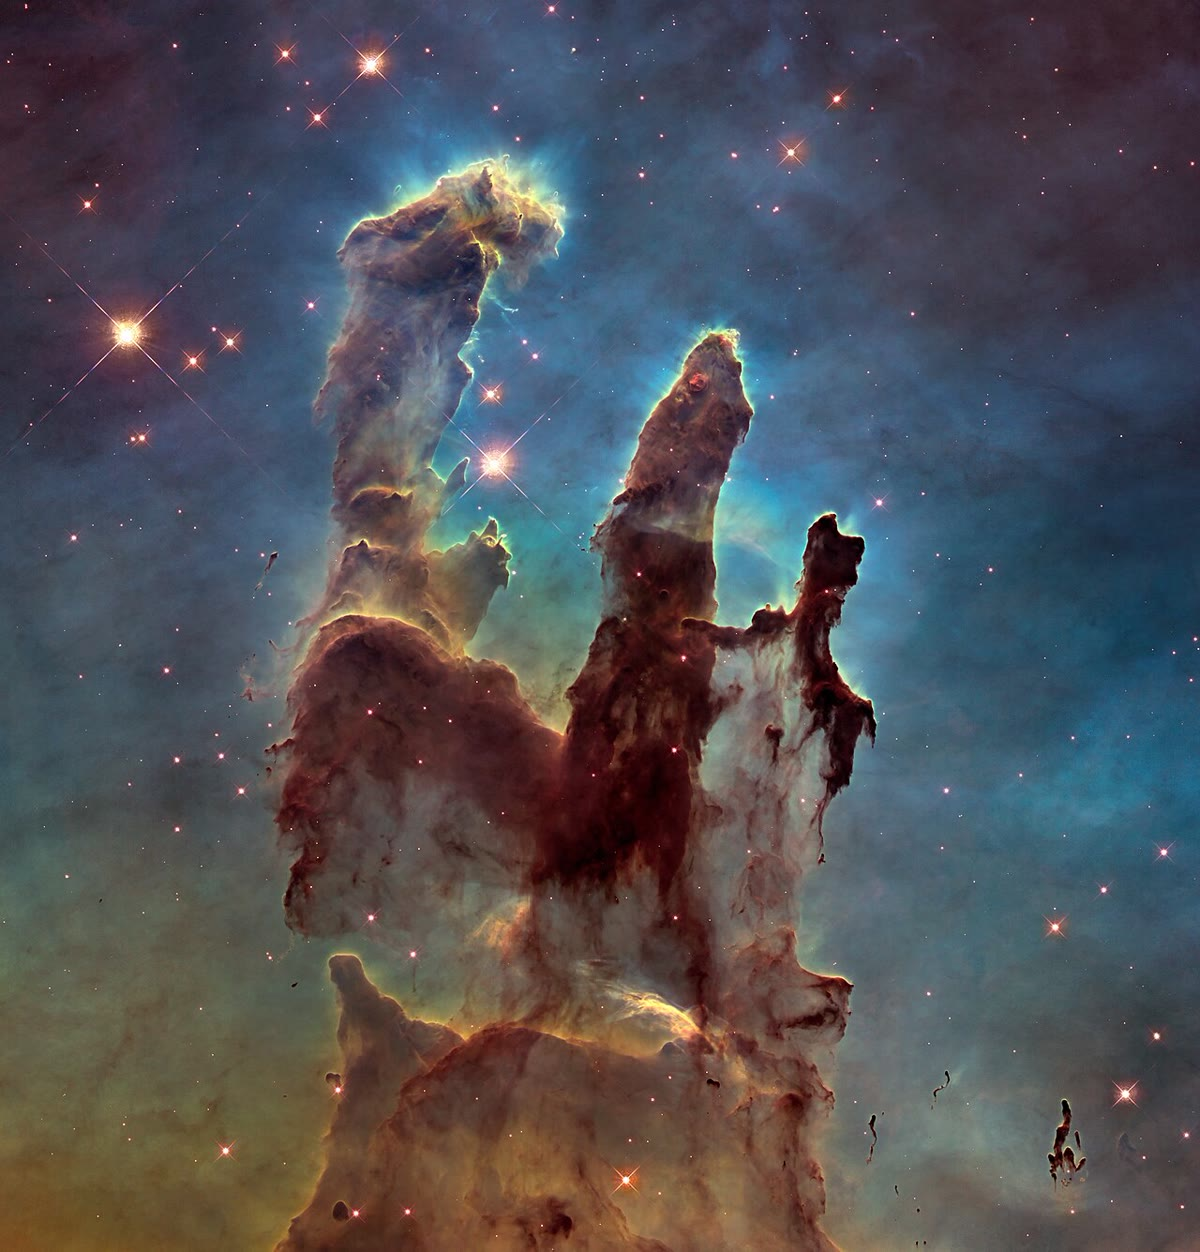
\includegraphics[width=\linewidth]{images/book4/b2-pillars-of-creation.jpg}
\end{minipage}\hfill
\begin{minipage}[c]{0.52\linewidth}
{\small Os ``Pilares da Criação'' na Nebulosa da Águia, fotografados pelo Telescópio
Espacial Hubble em luz visível. As colunas são gás molecular frio e denso e
poeira, com anos-luz de comprimento, erodidas e iluminadas de cima pela luz ultravioleta de
estrelas jovens de grande massa situadas fora da imagem; a poeira as torna opacas. Pequenas
condensações em suas pontas estão formando estrelas. NASA, ESA e Hubble
Heritage Team (STScI/AURA), domínio público.}
\end{minipage}
\end{omfigure}

\section{Colapso gravitacional}

Uma nuvem é um equilíbrio entre duas energias: a energia térmica de seu gás,
que empurra para fora, e sua energia gravitacional, que puxa para dentro. A
segunda cresce mais depressa com a massa que a primeira; acima de uma certa massa, a gravidade
vence.

\begin{proposition}[Energia gravitacional de uma esfera homogênea]
\label{prop:b2:ism-star-formation:grav-energy}
Uma esfera de densidade uniforme, de massa $M$ e raio $R$, tem a
energia potencial gravitacional
\[
  U = -\frac{3}{5}\,\frac{G M^2}{R}.
\]
\end{proposition}

\begin{proof}
Construa-se a esfera camada por camada. Quando seu raio é $r$, ela tem a massa
$m(r) = M r^3/R^3$; trazer do infinito até sua superfície uma camada de espessura $\mathrm dr$, de massa
$\mathrm dm = 3M r^2\,\mathrm dr/R^3$, libera
a energia $G m(r)\,\mathrm dm/r$, porque uma esfera atrai, do lado de fora, como se
sua massa estivesse em seu centro (o teorema das cascas, física). Logo
\[
  U = -\int_0^R \frac{G}{r}\,\frac{M r^3}{R^3}\,\frac{3 M r^2}{R^3}\,\mathrm dr
    = -\frac{3 G M^2}{R^6}\int_0^R r^4\,\mathrm dr = -\frac{3}{5}\,\frac{G M^2}{R}.
  \qedhere
\]
\end{proof}

Um corpo autogravitante em equilíbrio obedece ao teorema do virial: em média
no tempo, o dobro de sua energia cinética mais sua energia gravitacional é nulo,
$2K + U = 0$ (física, terceiro ano universitário, onde ele é deduzido das
equações do movimento). Para uma nuvem em repouso, $K$ é a energia térmica de suas
partículas. Se $2K > |U|$, o gás se expande; se $2K < |U|$, a gravidade não encontra
equilíbrio que se oponha a ela, e a nuvem se contrai.

\begin{proposition}[Critério de Jeans]\label{prop:b2:ism-star-formation:jeans}
Uma nuvem homogênea e isotérmica de temperatura $T$ e densidade $\rho$, formada de
partículas de massa média $\mu m_u$, colapsa sob a própria gravidade se sua massa
excede a \emph{\omterm{def:b2:ism-star-formation:jeans}{massa de Jeans}}
\[
  M_J = \left(\frac{5 k_{\mathrm B} T}{G\mu m_u}\right)^{3/2}
        \left(\frac{3}{4\pi\rho}\right)^{1/2},
\]
ou, de modo equivalente, se seu raio excede o \emph{\omterm{def:b2:ism-star-formation:jeans}{comprimento de Jeans}}
\[
  R_J = \left(\frac{15 k_{\mathrm B} T}{4\pi G\mu m_u\,\rho}\right)^{1/2}.
\]
Este é o \emph{critério de Jeans}\index{critério de Jeans}.
\end{proposition}

\begin{proof}
A nuvem contém $N = M/(\mu m_u)$ partículas, com a energia térmica
$K = \tfrac32 N k_{\mathrm B}T = \tfrac32 M k_{\mathrm B}T/(\mu m_u)$. Pela
\cref{prop:b2:ism-star-formation:grav-energy}, ela colapsa se
$2K < \tfrac35 GM^2/R$, isto é,
\[
  \frac{3 M k_{\mathrm B} T}{\mu m_u} < \frac{3}{5}\,\frac{G M^2}{R}
  \iff M > \frac{5 k_{\mathrm B} T}{G \mu m_u}\, R .
\]
Elimine-se $R$ com $M = \tfrac43\pi R^3\rho$, isto é, $R = (3M/4\pi\rho)^{1/3}$:
$M^{2/3} > \frac{5 k_{\mathrm B}T}{G\mu m_u}\,(3/4\pi\rho)^{1/3}$, e elevar
os dois membros à potência $3/2$ dá $M > M_J$. Eliminando-se $M$ em vez disso,
$\tfrac43\pi R^3\rho > 5 k_{\mathrm B}T R/(G\mu m_u)$ dá $R^2 > 15
k_{\mathrm B}T/(4\pi G\mu m_u\rho)$, isto é, $R > R_J$.
\end{proof}

\begin{definition}[Massa de Jeans, comprimento de Jeans]\label{def:b2:ism-star-formation:jeans}
A \emph{massa de Jeans}\index{massa de Jeans} $M_J$ e o \emph{comprimento
de Jeans}\index{comprimento de Jeans} $R_J$ de um gás de temperatura e densidade dadas
são a massa e o raio acima dos quais uma esfera homogênea desse gás
colapsa sob a própria gravidade (\cref{prop:b2:ism-star-formation:jeans}).
\end{definition}

A \omterm{def:b2:ism-star-formation:jeans}{massa de Jeans} cresce como $T^{3/2}$ e cai como $\rho^{-1/2}$: o gás frio e denso
é o que colapsa com mais facilidade. Em uma \omterm{def:b2:ism-star-formation:molecular-cloud}{nuvem molecular}, a massa média por partícula é
$\mu = 2.33$ unidades de massa atômica: hidrogênio molecular com um átomo de hélio para
cada cinco moléculas, aproximadamente. A \qty{10}{K} e $10^4$ partículas por centímetro
cúbico, $\rho = \mu m_u n = \qty{3.87e-17}{kg.m^{-3}}$ e
$M_J = 5.5$ massas solares, dentro de um \omterm{def:b2:ism-star-formation:jeans}{comprimento de Jeans} de \qty{0.13}{\parsec}:
a massa e o tamanho de um \omterm{def:b2:ism-star-formation:molecular-cloud}{núcleo denso}. Na densidade média de uma nuvem escura,
$100$ partículas por centímetro cúbico, a \omterm{def:b2:ism-star-formation:jeans}{massa de Jeans} é dez vezes maior, 55
massas solares, e uma nuvem de \num{24000} massas solares como a de Touro contém
centenas delas (figura abaixo).
% ledger: kauffmann:mu, nist:u, const:kB, const:G, sun:mass, goldsmith:taurus-mass

\begin{omfigure}
\begin{tabular}{@{}c@{\hspace{3mm}}c@{}}
\begin{tikzpicture}
\begin{axis}[omrecord, width=0.455\linewidth, height=6.0cm, xmode=log, ymode=log,
  xmin=10, xmax=1e7, ymin=0.05, ymax=1e4,
  xlabel={$n$ (\unit{cm^{-3}})}, ylabel={massa de Jeans (massas solares)},
  tick label style={font=\scriptsize}, label style={font=\small},
  legend style={font=\scriptsize, at={(0.97,0.97)}, anchor=north east, draw=none, fill=white, fill opacity=0.85}]
\fill[blue!12] (axis cs:1e4,0.5) rectangle (axis cs:1e5,5);
\node[font=\scriptsize, blue!50!black, anchor=north east] at (axis cs:1e5,0.5) {núcleos densos};
\addplot[very thick, blue!70!black] table[x=n, y=MJ10] {figdata/out/bachelor-2-jeans-jeans.dat};
\addlegendentry{\qty{10}{K}}
\addplot[very thick, orange!80!black] table[x=n, y=MJ20] {figdata/out/bachelor-2-jeans-jeans.dat};
\addlegendentry{\qty{20}{K}}
\addplot[very thick, red!75!black] table[x=n, y=MJ50] {figdata/out/bachelor-2-jeans-jeans.dat};
\addlegendentry{\qty{50}{K}}
\end{axis}
\end{tikzpicture}
&
\begin{tikzpicture}
\begin{axis}[omrecord, width=0.455\linewidth, height=6.0cm, xmode=log, ymode=log,
  xmin=10, xmax=1e7, ymin=0.01, ymax=20,
  xlabel={$n$ (\unit{cm^{-3}})}, ylabel={tempo de queda livre (Myr)},
  tick label style={font=\scriptsize}, label style={font=\small}]
\addplot[very thick, black!70] table[x=n, y=tff_Myr] {figdata/out/bachelor-2-jeans-tff.dat};
\fill[blue!12] (axis cs:1e4,0.05) rectangle (axis cs:1e5,0.5);
\addplot[very thick, black!70] table[x=n, y=tff_Myr] {figdata/out/bachelor-2-jeans-tff.dat};
\node[font=\scriptsize, blue!50!black, anchor=north] at (axis cs:3.2e4,0.05) {núcleos};
\end{axis}
\end{tikzpicture}
\\[2pt]
{\small (a) \omterm{def:b2:ism-star-formation:jeans}{Massa de Jeans}} & {\small (b) \omterm{def:b2:ism-star-formation:free-fall}{tempo de queda livre}}
\end{tabular}

\par\smallskip{\small (a) A \omterm{def:b2:ism-star-formation:jeans}{massa de Jeans} em função da densidade de partículas para três
temperaturas ($\mu = 2.33$). O retângulo sombreado marca as massas e densidades dos
\omterm{def:b2:ism-star-formation:molecular-cloud}{núcleos densos} observados: a \qty{10}{K}, sua massa é próxima da \omterm{def:b2:ism-star-formation:jeans}{massa de Jeans}. (b) O
\omterm{def:b2:ism-star-formation:free-fall}{tempo de queda livre} da \cref{prop:b2:ism-star-formation:free-fall}: um terço de milhão
de anos com $10^4$ partículas por centímetro cúbico, dez vezes mais com $10^2$.}
\end{omfigure}

Uma nuvem que começa a colapsar fica mais densa, e sua \omterm{def:b2:ism-star-formation:jeans}{massa de Jeans} cai como
$\rho^{-1/2}$ enquanto ela permanece fria, o que acontece enquanto ela consegue irradiar o
calor da compressão. Partes da nuvem tornam-se então instáveis por conta própria
e colapsam separadamente: a nuvem se \emph{fragmenta}. É por isso que as estrelas se formam
em grupos e que suas massas são pequenas comparadas com as das nuvens que as
originam. A fragmentação cessa quando o gás fica denso demais para deixar sua radiação
escapar: o calor da compressão fica aprisionado, a temperatura sobe e a
\omterm{def:b2:ism-star-formation:jeans}{massa de Jeans} para de cair.

Quanto tempo dura um colapso? Se a pressão for desprezível, cada camada da
nuvem cai livremente em direção ao centro.

\begin{proposition}[Tempo de queda livre]\label{prop:b2:ism-star-formation:free-fall}
Uma esfera homogênea de densidade $\rho$, inicialmente em repouso e sem pressão,
colapsa até seu centro no tempo
\[
  t_{\mathrm{ff}} = \left(\frac{3\pi}{32\,G\rho}\right)^{1/2},
\]
independente de seu raio.
\end{proposition}

\begin{proof}
Considere-se uma partícula em repouso à distância $R$ do centro, na
superfície da esfera. As camadas internas a ela caem mais depressa ou junto com ela, nunca
atrás, de modo que a massa $M = \tfrac43\pi R^3\rho$ que a atrai permanece a mesma
durante todo o percurso. Sua trajetória é uma órbita de Kepler degenerada: uma elipse achatada até virar
um segmento de reta, com a extremidade mais distante em $R$ e o centro de atração na
outra extremidade, de modo que seu semieixo maior é $a = R/2$. Cair da extremidade distante
até o centro leva meio período; pela terceira lei de Kepler,
\[
  t_{\mathrm{ff}} = \frac12\cdot 2\pi\sqrt{\frac{(R/2)^3}{GM}}
  = \pi\sqrt{\frac{R^3}{8\,G\cdot\frac43\pi R^3\rho}}
  = \sqrt{\frac{3\pi}{32\,G\rho}} .
\]
$R$ se cancela: todas as camadas de uma esfera homogênea chegam ao centro no mesmo
instante.
\end{proof}

\begin{definition}[Tempo de queda livre]\label{def:b2:ism-star-formation:free-fall}
O \emph{tempo de queda livre}\index{tempo de queda livre} de um gás de densidade $\rho$ é
$t_{\mathrm{ff}} = (3\pi/32G\rho)^{1/2}$, o tempo que uma esfera homogênea com essa
densidade levaria para colapsar apenas sob a própria gravidade.
\end{definition}

Para um \omterm{def:b2:ism-star-formation:molecular-cloud}{núcleo denso} de $10^4$ partículas por centímetro cúbico, o \omterm{def:b2:ism-star-formation:free-fall}{tempo de queda livre}
é de \qty{0.34}{Myr}; para uma nuvem escura inteira, de $10^2$, \qty{3.4}{Myr}. Se todas as
\omterm{def:b2:ism-star-formation:molecular-cloud}{nuvens moleculares} da Galáxia colapsassem em um \omterm{def:b2:ism-star-formation:free-fall}{tempo de queda livre} e se transformassem em
estrelas, a Galáxia formaria estrelas muito mais depressa do que forma: em Touro, o gás efetivamente transformado
em estrelas nos últimos três milhões de anos é cerca de um por cento da nuvem. As
nuvens são contidas por movimentos turbulentos e por campos magnéticos que a
fração ionizada do gás arrasta consigo, e a maior parte de seu gás é dispersa pelos
ventos e pela luz das primeiras estrelas de grande massa antes de poder colapsar: daí
a baixa eficiência medida em Touro.
% ledger: bt07:tff

\begin{history}[James Jeans]
James Jeans (1877--1946) publicou em 1902 a análise da estabilidade de um
gás sob a própria gravidade da qual descendem a massa e o \omterm{def:b2:ism-star-formation:jeans}{comprimento de Jeans}. Ele
estudou o crescimento de pequenas ondas de densidade em um gás homogêneo infinito e
descobriu que as ondas mais longas que um comprimento crítico não são contidas pela pressão,
mas crescem: o gás se divide em condensações com aproximadamente esse tamanho. Seu comprimento
crítico difere do raio encontrado acima apenas por um fator numérico; a
física, gravidade contra pressão térmica, é a mesma.
\end{history}

\section{Protoestrelas}

O colapso de um núcleo não é homogêneo. O centro, um pouco mais denso, cai
primeiro; ali se forma um objeto pequeno, denso e quente, que cresce engolindo o gás
que continua a chover sobre ele.

\begin{definition}[Protoestrela]\label{def:b2:ism-star-formation:protostar}
Uma \emph{protoestrela}\index{protoestrela} é uma estrela em formação que ainda
ganha a maior parte de sua massa por acreção do gás de seu núcleo de origem; ela
brilha pela energia que o gás em queda libera, e não por fusão nuclear.
\end{definition}

Com que rapidez cresce uma \omterm{def:b2:ism-star-formation:protostar}{protoestrela}? Um núcleo prestes a colapsar contém cerca de uma \omterm{def:b2:ism-star-formation:jeans}{massa de Jeans}
e cai em cerca de um \omterm{def:b2:ism-star-formation:free-fall}{tempo de queda livre}, de modo que a massa chega a uma taxa da ordem de
$M_J/t_{\mathrm{ff}}$.

\begin{proposition}[Taxa de acreção de uma protoestrela]
\label{prop:b2:ism-star-formation:accretion}
Seja $c_s = (k_{\mathrm B}T/\mu m_u)^{1/2}$ a velocidade do som isotérmica
do gás de um núcleo. A razão entre a \omterm{def:b2:ism-star-formation:jeans}{massa de Jeans} e o \omterm{def:b2:ism-star-formation:free-fall}{tempo de queda livre} não
depende da densidade, e
\[
  \frac{M_J}{t_{\mathrm{ff}}} \approx 10\,\frac{c_s^3}{G}:
\]
uma \omterm{def:b2:ism-star-formation:protostar}{protoestrela} cresce a uma taxa da ordem de $c_s^3/G$, fixada apenas pela temperatura de seu
núcleo.
\end{proposition}

\begin{proof}
Com $k_{\mathrm B}T/(\mu m_u) = c_s^2$, $M_J = 5^{3/2}\,c_s^3\,G^{-3/2}
(3/4\pi\rho)^{1/2}$ e $t_{\mathrm{ff}} = (3\pi/32)^{1/2}(G\rho)^{-1/2}$, de modo que
\[
  \frac{M_J}{t_{\mathrm{ff}}} = 5^{3/2}\left(\frac{3}{4\pi}\right)^{1/2}
  \left(\frac{32}{3\pi}\right)^{1/2}\frac{c_s^3}{G}
  = 11.18\times0.489\times1.84\,\frac{c_s^3}{G} \approx 10\,\frac{c_s^3}{G},
\]
em que $\rho$ se cancelou. O fator depende da forma do núcleo;
modelos de núcleos cuja densidade decresce para fora, como se observa, dão taxas
mais próximas do próprio $c_s^3/G$.
\end{proof}

A \qty{10}{K}, $c_s = \qty{0.19}{km.s^{-1}}$ e $c_s^3/G$ vale
\num{1.6e-6} massas solares por ano: uma estrela como o Sol se forma em cerca de
\num{600000} anos, um tempo comparável ao \omterm{def:b2:ism-star-formation:free-fall}{tempo de queda livre} de seu núcleo.
Em um núcleo mais quente, a \qty{20}{K}, a taxa é $2^{3/2} = 2.8$ vezes maior.

\begin{omfigure}
\begin{tikzpicture}[font=\scriptsize]
% panel 1: core
\begin{scope}
\shade[inner color=gray!70, outer color=gray!10] (0,0) circle (1.0);
\node[align=center] at (0,-1.45) {(1) núcleo denso\\$\sim\qty{0.1}{pc}$, \qty{10}{K}};
\end{scope}
% panel 2: collapse with infall arrows
\begin{scope}[xshift=3.0cm]
\shade[inner color=gray!80, outer color=gray!10] (0,0) circle (0.9);
\foreach \a in {0,45,...,315} \draw[-{Stealth[length=1.6mm]}, black!70] (\a:0.85) -- (\a:0.3);
\fill[orange!90!red] (0,0) circle (0.07);
\node[align=center] at (0,-1.45) {(2) colapso\\$t_{\mathrm{ff}} \sim \qty{0.1}{Myr}$};
\end{scope}
% panel 3: protostar with disc and outflow
\begin{scope}[xshift=6.0cm]
\fill[gray!25] (0,0) ellipse (0.9 and 0.6);
\fill[brown!55] (0,0) ellipse (0.75 and 0.12);
\fill[orange!90!red] (0,0) circle (0.08);
\fill[blue!25] (0,0.1) -- (-0.22,0.95) -- (0.22,0.95) -- cycle;
\fill[blue!25] (0,-0.1) -- (-0.22,-0.95) -- (0.22,-0.95) -- cycle;
\node[align=center] at (0,-1.45) {(3) protoestrela, disco\\e fluxo bipolar, $\sim\qty{0.5}{Myr}$};
\end{scope}
% panel 4: T Tauri with disc
\begin{scope}[xshift=9.0cm]
\fill[brown!55] (0,0) ellipse (0.85 and 0.1);
\fill[yellow!80!orange] (0,0) circle (0.1);
\draw[blue!40, thick] (0,0.15) -- (0,0.6); \draw[blue!40, thick] (0,-0.15) -- (0,-0.6);
\node[align=center] at (0,-1.45) {(4) estrela T Tauri\\e disco, 1--\qty{5}{Myr}};
\end{scope}
% panel 5: planetary system
\begin{scope}[xshift=12.0cm]
\fill[yellow!80!orange] (0,0) circle (0.12);
\foreach \r in {0.3,0.5,0.8} \draw[black!40] (0,0) ellipse ({\r} and {0.4*\r});
\fill (0.3,0) circle (0.03); \fill (-0.5,0.03) circle (0.035); \fill (0.8,0.05) circle (0.06);
\node[align=center] at (0,-1.45) {(5) estrela da sequência\\principal e planetas};
\end{scope}
\foreach \x in {1.4,4.4,7.4,10.4} \draw[-{Stealth}, thick, black!60] (\x,0) -- (\x+0.25,0);
\end{tikzpicture}

\par\smallskip{\small De um \omterm{def:b2:ism-star-formation:molecular-cloud}{núcleo denso} a um sistema planetário (esquema, fora de escala).
(1) Um núcleo frio próximo da \omterm{def:b2:ism-star-formation:jeans}{massa de Jeans}. (2) Seu centro colapsa primeiro e uma \omterm{def:b2:ism-star-formation:protostar}{protoestrela}
se forma. (3) A \omterm{def:b2:ism-star-formation:protostar}{protoestrela} cresce por acreção através de um disco, enquanto um \omterm{def:b2:ism-star-formation:t-tauri}{fluxo bipolar}
limpa o gás ao longo do eixo de rotação. (4) Desaparecido o envelope, uma \omterm{def:b2:ism-star-formation:t-tauri}{estrela T Tauri}, ainda
em contração, está cercada por seu disco. (5) O disco se dispersou; o que resta de
seus sólidos são planetas. Tempos tirados das estimativas de queda livre e de acreção do texto
e das durações de vida dos discos da última seção.}
\end{omfigure}

Enquanto acreta, a \omterm{def:b2:ism-star-formation:protostar}{protoestrela} brilha pela energia do gás em queda. Uma vez
esgotado o envelope, ela continua a brilhar, ainda sem fusão,
contraindo-se.

\begin{proposition}[A contração alimenta uma estrela jovem]
\label{prop:b2:ism-star-formation:contraction}
Uma esfera de gás autogravitante em equilíbrio que se contrai lentamente irradia
metade da energia gravitacional que libera e guarda a outra metade como calor:
ela fica mais quente enquanto perde energia.
\end{proposition}

\begin{proof}
Em equilíbrio, o teorema do virial dá $2K + U = 0$, de modo que a energia total é
$E = K + U = U/2$. Se o raio diminui, $U$ diminui de uma quantidade
$\Delta < 0$; então $E$ varia de $\Delta/2$, que é a energia irradiada
para fora, e $K = -U/2$ varia de $-\Delta/2 > 0$: a energia térmica, e portanto
a temperatura, aumentam da outra metade.
\end{proof}

\begin{definition}[Escala de tempo de Kelvin--Helmholtz]\label{def:b2:ism-star-formation:kh-time}
A \emph{escala de tempo de Kelvin--Helmholtz}\index{escala de tempo de Kelvin--Helmholtz}
de uma estrela de massa $M$, raio $R$ e luminosidade $L$ é
$t_{\mathrm{KH}} = GM^2/(RL)$, a ordem de grandeza do tempo durante o qual
a contração sozinha consegue fornecer sua luminosidade.
\end{definition}

Para o Sol atual, $t_{\mathrm{KH}} = \qty{31}{Myr}$: muito menos que sua
idade, e é por isso que o Sol precisa queimar hidrogênio. Para uma estrela jovem de uma massa
solar, com o dobro do raio do Sol e o dobro de sua luminosidade, são \qty{8}{Myr}
(\cref{exo:b2:ism-star-formation:6}). A contração termina quando o centro fica quente o bastante para que a fusão do hidrogênio
forneça a luminosidade: a estrela chega à sequência principal (como lembrado no início do capítulo).
% ledger: sun:mass, sun:R, sun:L, const:G

\begin{definition}[Estrela T Tauri, fluxo bipolar]\label{def:b2:ism-star-formation:t-tauri}
Uma \emph{estrela T Tauri}\index{estrela T Tauri} é uma estrela jovem de menos de cerca de
duas massas solares que já se livrou de seu envelope e se tornou visível, mas que ainda não
chegou à sequência principal: ela brilha por contração, varia de
brilho e em geral está cercada por um disco do qual ainda
acreta matéria. Um \emph{fluxo bipolar}\index{fluxo bipolar} é um par de jatos
ou ventos rápidos de gás ejetados por uma estrela jovem em sentidos opostos ao longo do
eixo de rotação de seu disco.
\end{definition}

Os \omterm{def:b2:ism-star-formation:t-tauri}{fluxos bipolares} levam embora parte do momento angular do gás que o disco
entrega à estrela, e limpam o envelope ao longo do eixo; a estrela de
HL Tauri, no fim de seu estágio protoestelar, produz um fluxo
fortemente colimado.
% ledger: alma:hltau

\section{Discos}

Um \omterm{def:b2:ism-star-formation:molecular-cloud}{núcleo denso} gira, lentamente: de um lado a outro de um núcleo, a velocidade do gás varia de alguns
décimos de quilômetro por segundo por parsec. Quando o núcleo colapsa, seu
momento angular se conserva, e a rotação lenta se torna rápida.

\begin{proposition}[Raio centrífugo]\label{prop:b2:ism-star-formation:centrifugal}
Um gás de momento angular específico $j$ (momento angular por unidade de massa)
que cai em direção a uma massa $M$ não consegue chegar ao centro: ele se instala em uma
órbita circular de raio
\[
  r_c = \frac{j^2}{G M}.
\]
\end{proposition}

\begin{proof}
Sem atrito, o momento angular do gás em queda se conserva, de modo que à
distância $r$ sua velocidade de rotação é $v = j/r$. O gás pode circular em $r$ se a
gravidade fornecer exatamente a aceleração centrípeta,
$GM/r^2 = v^2/r = j^2/r^3$, isto é, em $r = j^2/(GM)$. Mais para dentro, a
aceleração centrípeta necessária, $j^2/r^3$, excede a atração da gravidade, e
o gás não consegue avançar.
\end{proof}

O gás que cai ao longo do eixo de rotação tem pouco momento angular e vai
direto para a estrela; o gás que cai no plano equatorial conserva sua
rotação. O gás que cai de lados opostos por trajetórias diferentes colide
acima e abaixo do plano equatorial, perde seu movimento vertical e
se acumula em um disco fino em rotação, de raio da ordem de $r_c$. Para um núcleo de
\qty{0.1}{pc} que dá uma volta em uns vinte milhões de anos, $r_c$ é de algumas
centenas de unidades astronômicas (\cref{exo:b2:ism-star-formation:11}): o tamanho dos discos observados.

\begin{definition}[Disco protoplanetário]\label{def:b2:ism-star-formation:disc}
Um \emph{disco protoplanetário}\index{disco protoplanetário} (ou
\emph{disco protoestelar}\index{disco protoestelar}) é o disco achatado de
gás e poeira em rotação quase kepleriana em torno de uma estrela jovem, formado pela
matéria de seu núcleo de origem que conservou momento angular demais para cair na
estrela; os planetas se formam nele.
\end{definition}

\begin{omfigure}
\begin{minipage}[c]{0.44\linewidth}
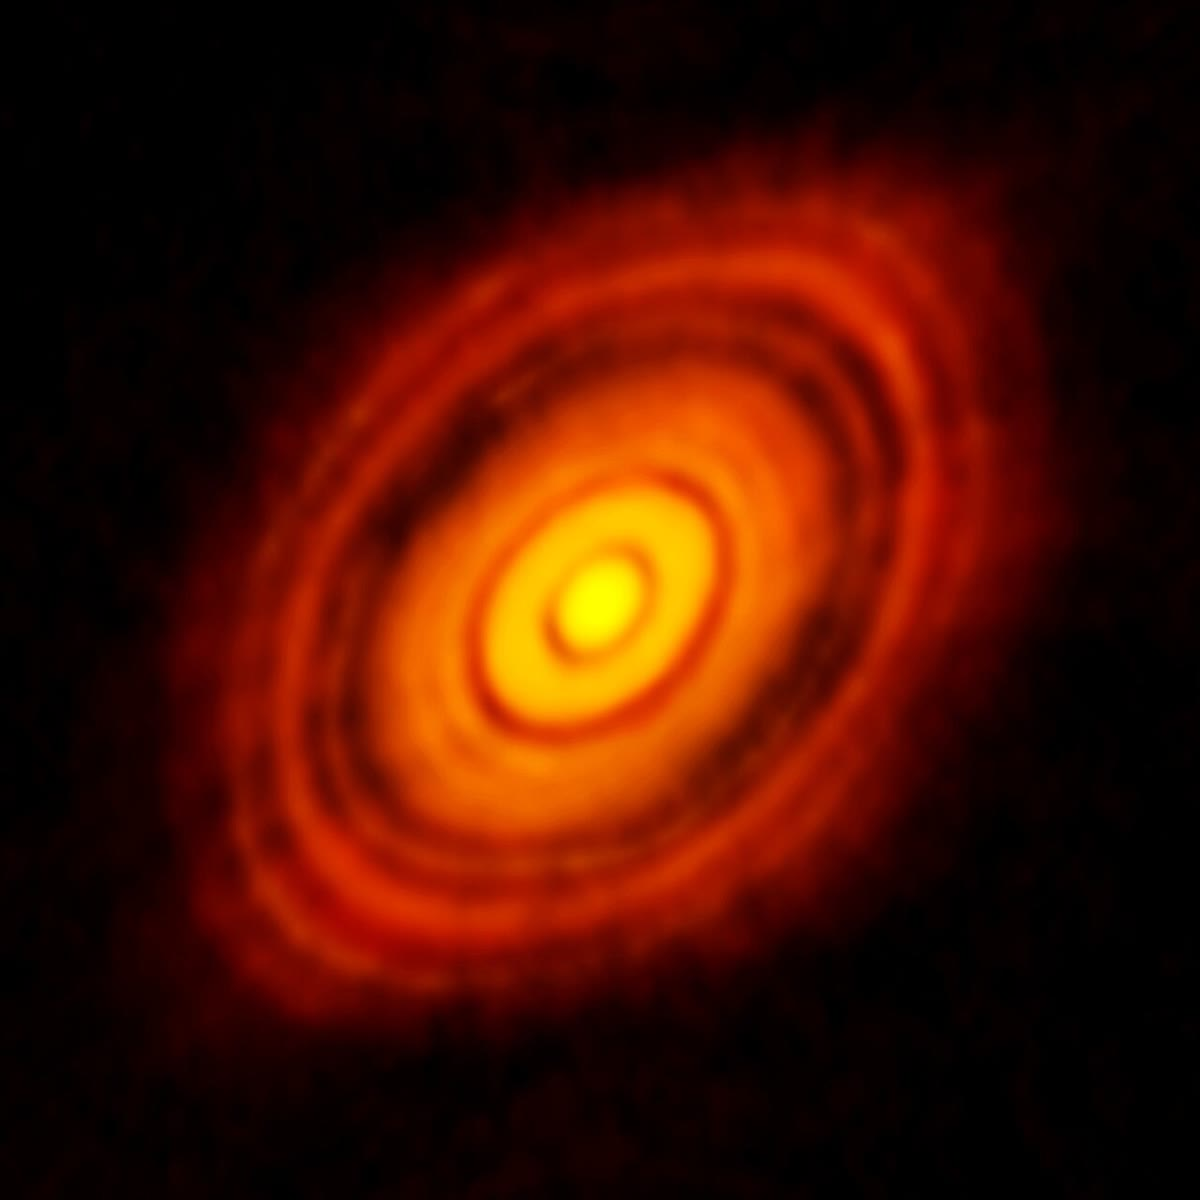
\includegraphics[width=\linewidth]{images/book4/b2-hl-tau-alma.jpg}
\end{minipage}\hfill
\begin{minipage}[c]{0.52\linewidth}
{\small O disco da estrela jovem HL Tauri, a \qty{140}{pc} de distância em Touro, fotografado
pelo interferômetro ALMA em um comprimento de onda de cerca de um milímetro, em que a poeira
fria brilha. O disco, com cerca de \qty{120}{au} de raio e visto inclinado de
\ang{47}, mostra anéis claros e escuros de algumas unidades astronômicas de largura; o
sistema tem no máximo um ou dois milhões de anos, e os anéis são interpretados como os
primeiros sinais de planetas abrindo caminho. ALMA (ESO/NAOJ/NRAO), CC BY 4.0.}
\end{minipage}
% ledger: alma:hltau
\end{omfigure}

O disco é aquecido pela estrela. Um grão à distância $r$ absorve a luz estelar
em sua seção transversal e irradia por toda a sua superfície.

\begin{proposition}[Temperatura de um grão iluminado por uma estrela]
\label{prop:b2:ism-star-formation:grain}
Um grão pequeno que se comporta como um corpo negro, à distância $r$ de uma estrela de
luminosidade $L$ e iluminado de um só lado, estabiliza-se à temperatura
\[
  T = \left(\frac{L}{16\pi\sigma r^2}\right)^{1/4},
\]
que decresce como $r^{-1/2}$.
\end{proposition}

\begin{proof}
Um grão esférico de raio $a$ intercepta a potência $\pi a^2\,L/(4\pi r^2)$
e, à temperatura $T$, irradia $4\pi a^2\sigma T^4$ por sua superfície.
No equilíbrio as duas são iguais: $T^4 = L/(16\pi\sigma r^2)$; $a$ se cancela.
\end{proof}

A \qty{1}{au} de uma estrela como o Sol, o grão está a \qty{278}{K}; a
\qty{5.2}{au}, onde Júpiter orbita, a \qty{122}{K}. O gelo de água se condensa onde
os grãos estão mais frios que cerca de \qty{180}{K} (as temperaturas de condensação são
as do \cref{ch:b2:planet-formation-meteorites}), isto é, além de cerca de
\qty{2.4}{au}: o primeiro indício da fronteira, a linha de neve, que separa
os planetas rochosos dos gelados. Um disco real é opaco, e seu plano médio fica protegido da luz estelar direta; a
proposição dá a ordem de grandeza certa e a inclinação certa para as
camadas superficiais que a estrela enxerga.
% ledger: lodders:tc-table

Os discos não duram. O excesso infravermelho, o brilho da poeira morna acima do que a estrela
sozinha emitiria, revela se uma estrela ainda tem um disco. Contar as estrelas
que têm esse excesso em aglomerados de idades diferentes dá a fração de estrelas
que conservam seu disco em função do tempo (figura abaixo): a maioria das estrelas tem um
ao nascer, metade já o perdeu por volta de três milhões de anos, e quase nenhuma
o conserva além de seis. Os gigantes gasosos, que precisam reunir seu gás no disco,
têm de se formar nesses poucos milhões de anos.
% ledger: haisch:disc-fractions, haisch:disc-lifetime

\begin{omfigure}
\begin{tikzpicture}
\begin{axis}[omrecord, width=0.8\linewidth, height=5.6cm, xmin=0, xmax=8.5, ymin=0, ymax=1.05,
  xlabel={idade do aglomerado (Myr)}, ylabel={fração de estrelas com disco},
  tick label style={font=\scriptsize}, label style={font=\small}, clip=false]
\addplot[thick, black!55, densely dashed] table[x=age, y=frac] {figdata/out/bachelor-2-jeans-discfit.dat};
\addplot[only marks, mark=*, mark size=1.8pt, blue!70!black,
  error bars/.cd, y dir=both, y explicit]
  table[x=age, y=frac, y error=err, restrict x to domain=0:10] {figdata/out/bachelor-2-jeans-discs.dat};
\node[font=\scriptsize, anchor=north west] at (axis cs:0.05,0.74) {NGC 2024};
\node[font=\scriptsize, anchor=south west] at (axis cs:1.55,0.86) {Trapézio};
\node[font=\scriptsize, anchor=south west] at (axis cs:2.35,0.71) {IC 348};
\node[font=\scriptsize, anchor=south west] at (axis cs:3.3,0.56) {NGC 2264};
\node[font=\scriptsize, anchor=south west] at (axis cs:5.1,0.15) {NGC 2362};
\node[font=\scriptsize, anchor=north east] at (axis cs:8.4,0.98) {(NGC 1960, \qty{30}{Myr}: $0.03$)};
\end{axis}
\end{tikzpicture}

\par\smallskip{\small Fração das estrelas de aglomerados jovens que mostram o excesso
infravermelho de um disco, em função da idade do aglomerado (com seu erro), segundo Haisch, Lada
e Lada (2001). A reta tracejada é a reta de mínimos quadrados ajustada aos cinco
aglomerados mais jovens: ela atinge $0.5$ em \qty{3.0}{Myr} e zero em \qty{6.1}{Myr}
(\cref{exo:b2:ism-star-formation:12}).}
\end{omfigure}

\begin{inthelab}[Ver através da poeira com ondas de rádio]
\begin{minipage}[t]{0.55\linewidth}\vspace{0pt}
O gás frio e a poeira são invisíveis aos telescópios ópticos, mas brilham em comprimentos de onda
milimétricos, nos quais a atmosfera só é transparente acima de locais altos e secos. Uma
antena de rádio do tamanho de uma casa resolve pouco nesses comprimentos de onda, por isso
os astrônomos combinam muitas: em um interferômetro, cada par de antenas, separadas
por uma linha de base, mede uma componente do padrão de brilho do céu, e
um computador monta a imagem a partir das centenas de pares que umas trinta antenas formam. A resolução é a de
um único telescópio tão largo quanto a linha de base mais longa: com antenas espalhadas por
\qty{15}{km}, o disco de HL Tauri foi fotografado com detalhes de algumas unidades astronômicas a
\qty{140}{pc}. Operadores deslocam as antenas em transportadores entre configurações,
e o correlacionador combina seus sinais em tempo real.
\end{minipage}\hfill
\begin{minipage}[t]{0.42\linewidth}\vspace{0pt}
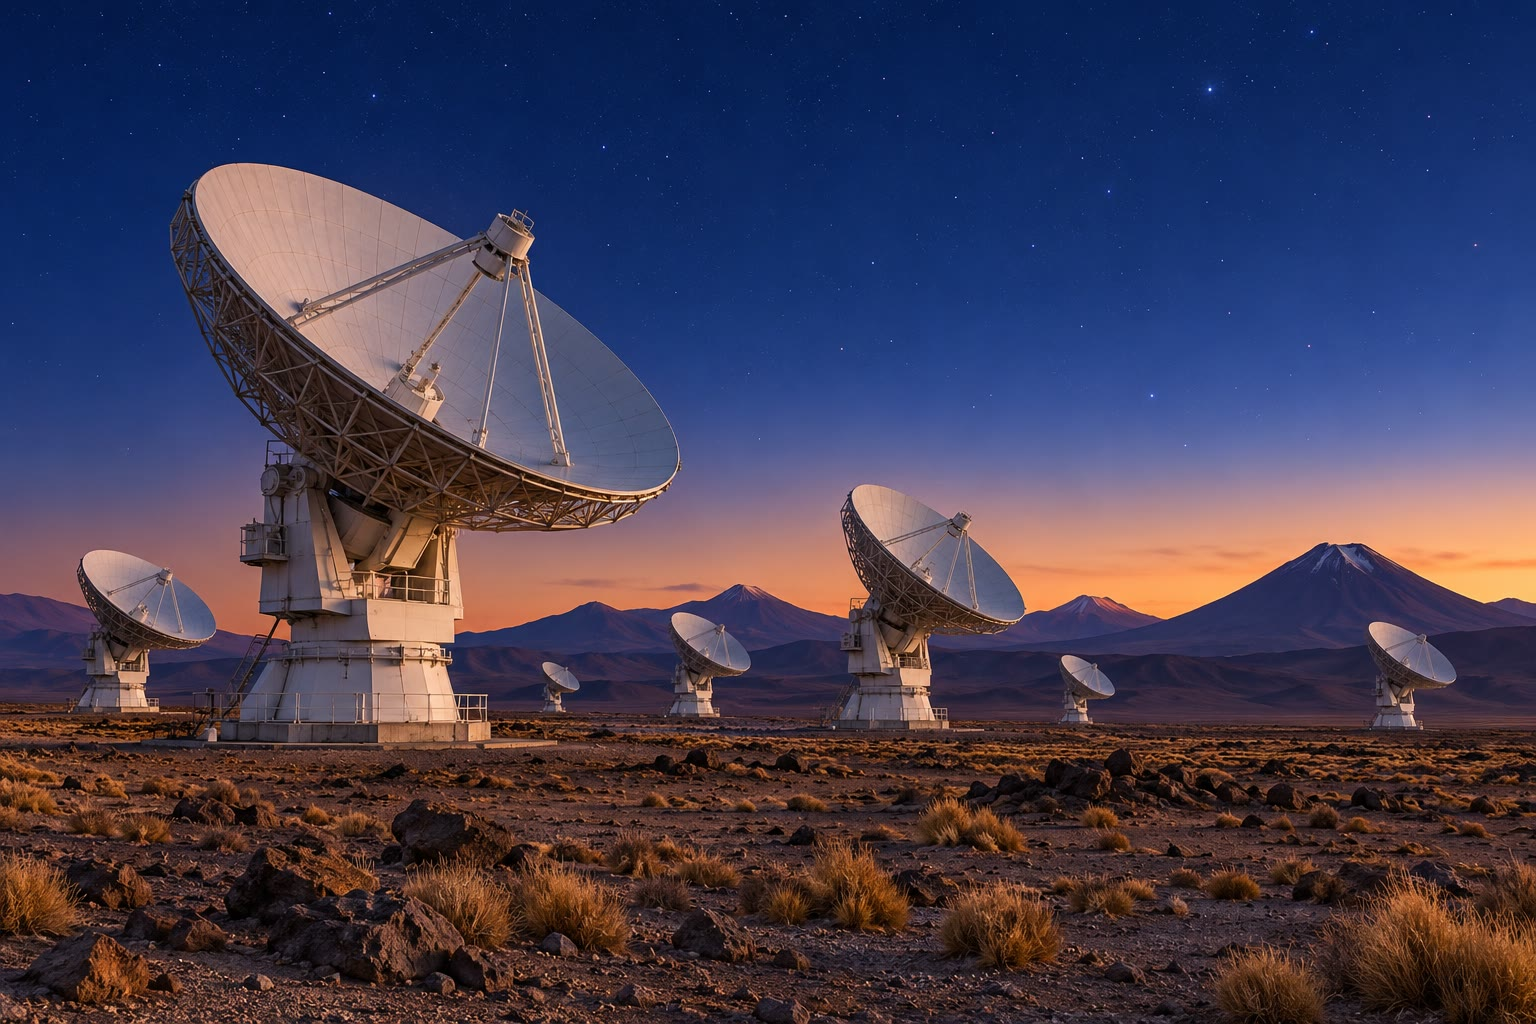
\includegraphics[width=\linewidth]{images/book4/ai/b2-radio-array.jpg}

{\scriptsize Um conjunto de antenas de rádio em um planalto desértico elevado ao entardecer
(ilustração gerada por IA).}
\end{minipage}
% ledger: alma:hltau, alma:baselines
\end{inthelab}

\section{Exercícios}

\begin{exercise}[$\star$]\label{exo:b2:ism-star-formation:1}
A densidade interestelar média perto do Sol é \qty{2.7e-24}{g.cm^{-3}}. Tomando
a massa de um átomo de hidrogênio como \qty{1.67e-24}{g}, calcule o número de átomos de
hidrogênio por centímetro cúbico. Compare com o número de moléculas por centímetro
cúbico do ar a \qty{101325}{Pa} e \qty{288}{K} ($n = P/k_{\mathrm B}T$).
% ledger: ferriere:mean-density, const:kB
\end{exercise}

\begin{exercise}[$\star$]\label{exo:b2:ism-star-formation:2}
Usando o valor $M_J = 5.46$ massas solares a \qty{10}{K} e $10^4$ partículas
por centímetro cúbico, e a dependência de $M_J$ com a densidade, calcule a \omterm{def:b2:ism-star-formation:jeans}{massa de
Jeans} a \qty{10}{K} e $10^2$ partículas por centímetro cúbico. Quantas \omterm{def:b2:ism-star-formation:jeans}{massas de
Jeans} contém a nuvem de Touro, de \num{24000} massas solares?
% ledger: goldsmith:taurus-mass
\end{exercise}

\begin{exercise}[$\star$]\label{exo:b2:ism-star-formation:3}
Calcule a velocidade do som isotérmica $c_s = (k_{\mathrm B}T/\mu m_u)^{1/2}$ do
gás molecular ($\mu = 2.33$, $m_u = \qty{1.661e-27}{kg}$) a \qty{10}{K} e a
\qty{100}{K}. Quanto tempo uma onda sonora leva para atravessar um núcleo de raio
\qty{0.1}{pc} a \qty{10}{K}, em milhões de anos?
% ledger: kauffmann:mu, nist:u, iau:parsec
\end{exercise}

\begin{exercise}[$\star$]\label{exo:b2:ism-star-formation:4}
Calcule o \omterm{def:b2:ism-star-formation:free-fall}{tempo de queda livre} de um \omterm{def:b2:ism-star-formation:molecular-cloud}{núcleo denso} de $10^5$ partículas por centímetro
cúbico e de uma nuvem escura de $10^2$ ($\mu = 2.33$). Qual colapsa
mais depressa, e por que fator?
\end{exercise}

\begin{exercise}[$\star\star$]\label{exo:b2:ism-star-formation:5}
Mostre que $M_J$ pode ser escrita $M_J = 5^{3/2}\,(3/4\pi)^{1/2}\,c_s^3\,G^{-3/2}\rho^{-1/2}$.
A temperatura fixa, por que fator a densidade de um núcleo precisa aumentar para reduzir
sua \omterm{def:b2:ism-star-formation:jeans}{massa de Jeans} à metade? A densidade fixa, por que fator muda a \omterm{def:b2:ism-star-formation:jeans}{massa de Jeans} se
o núcleo se aquece de \qty{10}{K} para \qty{20}{K}?
\end{exercise}

\begin{exercise}[$\star\star$]\label{exo:b2:ism-star-formation:6}
Uma estrela jovem tem a massa do Sol, o dobro de seu raio e o dobro de sua luminosidade
($M_\odot = \qty{1.989e30}{kg}$, $R_\odot = \qty{6.96e8}{m}$,
$L_\odot = \qty{3.83e26}{W}$). Calcule seu tempo de Kelvin--Helmholtz em milhões de
anos e compare-o com as durações de vida dos discos.
% ledger: sun:mass, sun:R, sun:L
\end{exercise}

\begin{exercise}[$\star\star$]\label{exo:b2:ism-star-formation:7}
Calcule a taxa de acreção $c_s^3/G$ de uma \omterm{def:b2:ism-star-formation:protostar}{protoestrela} em um núcleo a \qty{10}{K}, em
massas solares por ano, e o tempo que ela leva para reunir uma massa solar. Mesmas
perguntas para um núcleo a \qty{20}{K}.
\end{exercise}

\begin{exercise}[$\star\star$]\label{exo:b2:ism-star-formation:8}
Com a \cref{prop:b2:ism-star-formation:grain} e $L_\odot = \qty{3.83e26}{W}$,
calcule a distância ao Sol, em unidades astronômicas, na qual um grão
atinge \qty{1300}{K}, perto da temperatura em que os silicatos comuns
se condensam (\cref{ch:b2:planet-formation-meteorites}), e
a temperatura de um grão à distância de Júpiter, \qty{5.2}{au}.
% ledger: sun:L, const:sigma, const:au
\end{exercise}

\begin{exercise}[$\star\star$]\label{exo:b2:ism-star-formation:9}
O gás do disco de HL Tauri gira em torno de uma estrela de cerca de \num{1.3} massas
solares. Calcule a velocidade kepleriana e o período orbital a \qty{100}{au}.
Se o sistema tem um milhão de anos, quantas voltas o gás a
\qty{100}{au} deu desde que a estrela se formou?
% ledger: alma:hltau
\end{exercise}

\begin{exercise}[$\star\star\star$]\label{exo:b2:ism-star-formation:10}
Determine a energia gravitacional de uma esfera de raio $R$ na qual a densidade
decresce como $\rho(r) = \rho_0 R/r$, e compare-a com a de uma esfera homogênea de
mesma massa e mesmo raio. Concentrar a massa em direção ao centro torna
a nuvem mais fácil ou mais difícil de sustentar por sua energia térmica?
\end{exercise}

\begin{exercise}[$\star\star\star$]\label{exo:b2:ism-star-formation:11}
Um núcleo de raio \qty{0.1}{pc} gira como um corpo rígido à velocidade angular
$\Omega = \qty{1e-14}{rad.s^{-1}}$. Calcule seu período de rotação, o momento angular
específico $j = \Omega R^2$ do gás em seu equador e o raio centrífugo
desse gás em torno de uma estrela de uma massa solar, em unidades astronômicas.
Por que o gás do interior do núcleo cai mais perto da estrela?
\end{exercise}

\begin{exercise}[$\star\star\star$]\label{exo:b2:ism-star-formation:12}
As frações de estrelas com disco dos cinco aglomerados mais jovens da figura da última
seção são $0.85$, $0.80$, $0.65$, $0.52$ e $0.12$ a 0.3, 1.5, 2.3, 3.2 e
\qty{5.0}{Myr}. Ajuste à mão uma reta de mínimos quadrados $f = a - bt$
(calcule as médias, depois $\sum(t - \bar t)(f - \bar f)$ e
$\sum(t - \bar t)^2$). Com que idade ela atinge um meio, e zero? Por que uma
reta é um modelo ruim além dessa idade?
% ledger: haisch:disc-fractions
\end{exercise}

\section{Problema: um núcleo na nuvem de Aldra}

\begin{problem}[{Problema de fim de semana --- a massa e a estabilidade de um núcleo denso lidas em um
mapa de poeira, o nascimento de sua protoestrela e o tamanho de seu disco}]
\label{pb:b2:ism-star-formation:1}
% values: calc/ch01.py
% ledger: kauffmann:mu, nist:u, iau:parsec, const:G, const:kB, sun:mass, sun:R, sun:L, const:au, const:sigma, bt07:cores, alma:hltau
A nuvem de Aldra é uma nuvem escura inventada. Um mapa milimétrico de sua poeira
mostra um núcleo redondo de raio \qty{0.08}{pc}, com uma densidade de coluna média de
$N(\ce{H2}) = \num{1.5e22}$ moléculas de hidrogênio por centímetro quadrado. Uma
linha da amônia dá a temperatura do gás, \qty{10}{K}, e um gradiente de
velocidade de \qty{0.4}{km.s^{-1}} por parsec de um lado a outro do núcleo, interpretado como rotação
de corpo rígido. Use $G = \qty{6.674e-11}{m^3.kg^{-1}.s^{-2}}$,
$k_{\mathrm B} = \qty{1.381e-23}{J.K^{-1}}$, $m_u = \qty{1.661e-27}{kg}$,
\qty{1}{pc} $= \qty{3.086e16}{m}$, \qty{1}{au} $= \qty{1.496e11}{m}$, um ano de
\qty{3.156e7}{s}, $M_\odot = \qty{1.989e30}{kg}$, $R_\odot = \qty{6.96e8}{m}$,
$L_\odot = \qty{3.83e26}{W}$, $\sigma = \qty{5.67e-8}{W.m^{-2}.K^{-4}}$; a
massa por molécula de hidrogênio, hélio incluído, é $2.8\,m_u$, e a massa média
por partícula, $2.33\,m_u$.

\medskip
\noindent\textbf{Parte I --- Massa e densidade.}
\begin{enumerate}
  \item Converta o raio do núcleo em metros.
  \item Calcule a massa por metro quadrado da coluna, $2.8\,m_u N$.
  \item Deduza a massa do núcleo, em quilogramas e em massas solares.
  \item Calcule seu volume e sua densidade média.
  \item Calcule o número de partículas por centímetro cúbico.
  \item Trata-se de um \omterm{def:b2:ism-star-formation:molecular-cloud}{núcleo denso} no sentido da tabela da segunda seção?
\end{enumerate}

\noindent\textbf{Parte II --- Estabilidade.}
\begin{enumerate}[resume]
  \item Calcule a \omterm{def:b2:ism-star-formation:jeans}{massa de Jeans} do gás do núcleo, em massas solares.
  \item Quantas \omterm{def:b2:ism-star-formation:jeans}{massas de Jeans} o núcleo contém? Ele é estável?
  \item Calcule o \omterm{def:b2:ism-star-formation:jeans}{comprimento de Jeans} e compare-o com o raio do núcleo.
  \item Qual seria a \omterm{def:b2:ism-star-formation:jeans}{massa de Jeans} se o gás estivesse a \qty{20}{K}? O
        núcleo ainda colapsaria?
  \item Calcule o \omterm{def:b2:ism-star-formation:free-fall}{tempo de queda livre} do núcleo, em milhares de anos.
  \item Compare-o com o tempo que uma onda sonora leva para atravessar o núcleo. Qual
        processo é mais rápido, e o que isso significa?
\end{enumerate}

\noindent\textbf{Parte III --- A protoestrela.}
\begin{enumerate}[resume]
  \item Calcule a velocidade do som no núcleo.
  \item Calcule a taxa de acreção $c_s^3/G$, em massas solares por ano.
  \item Calcule o tempo necessário para reunir uma massa solar a essa taxa.
  \item Se um terço do núcleo acaba em estrelas, quantas estrelas de uma massa solar
        ele pode formar?
  \item Desaparecido o envelope, a estrela tem uma massa solar, três raios
        solares e quatro luminosidades solares. Calcule seu tempo de Kelvin--Helmholtz.
  \item Ele é mais longo ou mais curto que o tempo de acreção? Que tipo de estrela
        ela é então?
\end{enumerate}

\noindent\textbf{Parte IV --- O disco.}
\begin{enumerate}[resume]
  \item Converta o gradiente de velocidade em uma velocidade angular $\Omega$, em
        \unit{rad.s^{-1}}.
  \item Calcule o momento angular específico $j = \Omega R^2$ do gás no
        equador do núcleo.
  \item Calcule seu raio centrífugo em torno de uma estrela de uma massa solar, em
        unidades astronômicas.
  \item Calcule a temperatura de um grão a \qty{1}{au} e a \qty{30}{au}
        de uma estrela de uma luminosidade solar.
  \item Onde fica a linha de neve desse disco, se o gelo de água sobrevive abaixo de
        \qty{180}{K}?
  \item Indique o tempo necessário para formar a estrela da pergunta 15, o número-chave
        deste problema, em milhares de anos, e compare-o com o
        \omterm{def:b2:ism-star-formation:free-fall}{tempo de queda livre} da pergunta 11.
\end{enumerate}
\end{problem}
